\documentclass[landscape]{article}
\usepackage{amssymb}
\usepackage[landscape]{geometry}
\usepackage{color}
\usepackage{graphicx}
\usepackage{tikz}
\usepackage{amsfonts, amstext, amsmath}
\usepackage{wrapfig}
\usepackage{float}
\usepackage[export]{adjustbox}
\usepackage{tcolorbox}
\usepackage{times}
\usepackage{anyfontsize}
\usepackage{tikz}
\usepackage{graphicx}
\usepackage{multicol}
\usetikzlibrary{calc,bayesnet,shapes.geometric,arrows,chains,matrix,positioning,scopes,calendar,decorations.markings,decorations.pathreplacing,intersections}
\usetikzlibrary{arrows.meta}

\makeatletter
\tikzset{join/.code=\tikzset{after node path={%
      \ifx\tikzchainprevious\pgfutil@empty\else(\tikzchainprevious)%
      edge[every join]#1(\tikzchaincurrent)\fi}}
}
%\tikzset{>=stealth',every on chain/.append style={join},
%  every join/.style={->}
%}

\newcommand{\inputTikZ}[2]{%  
     \scalebox{#1}{\input{#2}}  
}

\newtcolorbox{mybox}{boxrule=6pt}

\def\argmax{\qopname\relax n{argmax}}
\def\s{\mathbf s}
\def\x{\mathbf x}
\def\u{\mathbf u}
\def\y{\mathbf y}
\def\d{\mathbf d}
\def\boldzero{\mathbf 0}
\def\pibold{\mbox{\boldmath $\pi$}}
\newcommand{\normal}[2]{\ensuremath{\mathcal{N}\left(#1,#2\right)}}
\newcommand{\given}{\mid}

\newenvironment{itemizeNoSymbol}{%
\renewcommand{\labelitemi}{}\begin{itemize}
\setlength{\itemsep}{1pt}
\setlength{\parskip}{0pt}
\setlength{\parsep}{0pt}}{\end{itemize}}


% set horizontal margins to center text (using current paperwidth &
% textwidth)
\newcommand{\equalmargins} {
\setlength{\oddsidemargin}{\paperwidth}
\addtolength{\oddsidemargin}{-\textwidth}
\setlength{\oddsidemargin}{0.5 \oddsidemargin}
\addtolength{\oddsidemargin}{-1in}
}

\setlength{\evensidemargin}{\oddsidemargin}

\renewcommand{\familydefault}{\sfdefault}

\input posterfonts.tex

% setup large (poster-sized) sheet
\setlength{\paperwidth}{841mm}
\setlength{\paperheight}{1189mm}
%\pdfpagewidth\paperwidth
%\pdfpageheight\paperheight
 
\setlength{\textwidth}{820mm}
\setlength{\textheight}{1170mm}
\setlength{\topmargin}{-.25truein}
 
\equalmargins
\setlength{\headsep}{0pt}
\setlength{\headheight}{0pt}

\pagestyle{empty}
\setlength{\parindent}{0mm}
\setlength{\parskip}{16pt}

% header style: title followed by a column-wide rule
\newcommand{\mysection}[1]{{\color[rgb]{.6,0,0}{\section*{{\LARGE #1}
        {\leaders\hrule height .2ex\hfill\kern0pt}}}}}

\begin{document}
\color{black}

% invisible rule is useful for spacing
\hrule width 0pt depth 0pt height 1pt

\begin{center}
  \HUGE
Examining models in theoretical neuroscience \\  with degenerate solution networks \\
  \Large %
  Sean R. Bittner$^{1}$, Alex T. Piet  $^{2}$, Chunyu A. Duan  $^{3}$, Agostina Palmigiano$^{1}$, Kenneth D. Miller$^{1}$, Carlos D. Brody  $^{2}$, and John P. Cunningham$^4$ \\
  \large
  $^{1}$Department of Neuroscience, Columbia University, $^{2}$ Princeton Neuroscience Institute, $^{3}$ Institute of Neuroscience, Chinese Academy of Sciences, and \\ $^{4}$Department of Statistics, Columbia University
\end{center}

\begin{tikzpicture}[remember picture,overlay]
  \node[anchor=north east,inner sep=0pt, scale=0.75] at ($(current page.north east)+(-2.5cm,-1.0cm)$) {
     
\includegraphics{figs/CU_logo}
  };
\end{tikzpicture}

%%%%%%%%%%%%%%%%%%%%%%%%%%%%%%
\begin{minipage}[c]{0.29\linewidth}

\mysection{Motivation}
\large
\begin{itemize}
\item Circuit models are often designed in the hopes of producing an emergent property observed in data (e.g., an oscillation, limit cycle, etc.)
\item However, the standard inference toolkit conditions on data, not this emergent property.
\item We develop degenerate solution networks (DSNs), which learns distributions over model parameters that produce a desired emergent behavior.
\item DSNs produce new insights into existing models and will become increasingly important as models get more complex.
\end{itemize}

\mysection{Example: biophysical model}
\begin{itemize}
\item The desire to make a neural model biologically realistic and interpretable is at odds with the tractability of its analysis. 
\end{itemize}
\begin{center}
{ \textbf{Stomatogastric ganglion (STG)}}
\large
\end{center}
\begin{multicols*}{2}
\begin{center}
\includegraphics[scale=0.65]{figs/STGCircuit_param.pdf}
\end{center}
\columnbreak
\begin{itemize}
\item This conductance-based biophysical model is a complex nonlinear dynamical system.
\item The hub neuron's firing rate settles into one of two regimes: fast ($f_1$, $f_2$) or slow ($s_1$, $s_2$) [1].
\end{itemize}
\end{multicols*}
\begin{itemize}
\item For some $g_{\text{synA}}$ and $g_{\text{el}}$, the entire network syncs at a frequency of 0.55Hz $\rightarrow$ an emergent property.
\end{itemize}
\begin{mybox}
\textbf{Question}: Which parameters result in the entire network syncing at roughly 0.55Hz? \\
\textbf{Classic approach}: Simulate the neural model and search for structure in the activity.
\begin{center}
\includegraphics[scale=0.65]{figs/classic_approach.pdf}
\end{center}
\textbf{DSN approach}: Learn a structured distribution on parameters producing the emergent property.
\begin{center}
\includegraphics[scale=0.75]{figs/dsn_approach.pdf}
\end{center}
\end{mybox}

\begin{multicols*}{2}
\begin{itemize}
\item The DSN Hessian shows sensitive and degenerate dimensions.
\end{itemize}
\columnbreak
\begin{center}
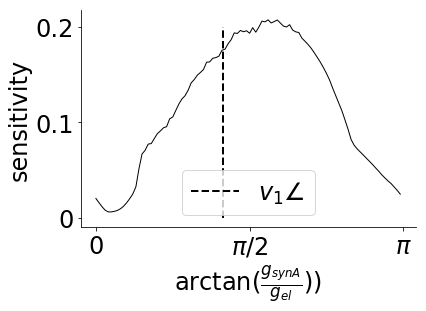
\includegraphics[scale=0.6]{figs/STG_sensitivity.png}
\end{center}
\end{multicols*}

\mysection{Methods}
{\LARGE \textbf{Deep probability distributions}}
\begin{itemize}
\item Deep probability distributions are obtained by optimizing deep networks to map (approximately) a simple random distribution to a target distribution.
\[z = f_l \circ f_{l-1} \circ ... \circ f_1 \circ \omega \]
\end{itemize}
\begin{center}
\adjincludegraphics[clip, trim={0 0 0 0},scale=1.3]{figs/DSN.pdf}
\end{center}
\begin{itemize}
\item \textbf{Max-entropy flow networks} are deep probability distributions that approximate maximum entropy distributions that satisfy sets of constraints [2].
\end{itemize}
{\Large
 \begin{equation*}
\argmax_{q_\theta \in Q} H(q_\theta) \text{\hspace{.4in} s.t. } E_{q_\theta} \left[T(z) \right] = \mu 
\end{equation*}}


\end{minipage}
\hspace{1cm} \begin{minipage}[c]{0.36\linewidth}
%%%%%%%%%%%%%%%%%%%%%%%%%%%%%%
\mysection{Degenerate solution networks (DSNs)}
\large
\begin{mybox}
\begin{itemize}
\item DSNs are deep probability distributions of parameters $z \sim q_\theta(z)$ yielding emergent property $\mathcal{B}: E_{z \sim q_\theta(z)} \left[ E_{p(x \mid z)} \left[T(x) \right] \right] = \mu$, for choice of model $p(x \mid z)$ and behavior $T(x)$.
\[q_\theta^*(z) = \mathop{\arg\,\max}\limits_{q_\theta \in Q} H(q_\theta(z)) \]
\[ \text{s.t.  } \mathcal{B}: E_{z \sim q_\theta}\left[ E_{x\sim p(x \mid z)}\left[T(x)\right] \right] = \mu \]
\item An equivalent conceptualization is that DSNs do posterior inference conditioned on an emergent property.
\end{itemize}
\begin{center}
\includegraphics[scale=0.55]{figs/DSN_panel1.pdf}
\end{center}
\textbf{Example: STG}
\begin{center}
\includegraphics[scale=0.65]{figs/DSN_panel2.pdf}
\end{center}
\begin{itemize}
\item This DSN optimized $\theta$ to produce a deep probabilistic distribution of model parameters $g_{\text{synA}}$ and $g_{\text{el}}$, which results in a 0.55Hz firing rate for each neuron with (0.025Hz)$^2$ variance.
\end{itemize}
 \end{mybox} 
 
 \vspace{1cm}
\mysection{Exploratory analyses of V1 model}
\vspace{-.8cm}
\begin{itemize}
\item Theoretical neuroscientists look to extend E-I dynamical models to four populations $\rightarrow$ E, P, S, and V.
\end{itemize}
\begin{center}
\includegraphics[scale=1.2]{figs/V1_panel1.pdf}
\end{center}
\begin{itemize}
\item Experimental evidence shows that the only mutually inhibitory pair (S and V) have a winner-take-all relationship [3].
\item We explored the S- and V-silenced regimes with DSNs.
\end{itemize}

\begin{center}
\includegraphics[scale=1.0]{figs/V1_panel2.pdf}
\end{center}

\begin{itemize}
\item The Hessian of the DSNs at $\gamma(W)=0$ gives eigvecs showing dims sensitive and degenerate w.r.t. inhibition stabilization.
\end{itemize}

\begin{center}
\includegraphics[scale=1.0]{figs/V1_panel3.pdf}
\end{center}

\begin{itemize}
\item We can look at how inhibition is distributed across multiple interneuron types across randomized solutions of $\gamma$ regimes.
\end{itemize}

\begin{center}
\includegraphics[scale=0.8]{figs/V1_panel4.pdf}
\end{center}

%\begin{center}
%\includegraphics[scale=1.0]{figs/V1_panel4.pdf}
%\end{center}
\end{minipage}
\hspace{1cm} \begin{minipage}[c]{0.29\linewidth}
%%%%%%%%%%%%%%%%%%%%%%%%%%%%%%
\mysection{Identifying learning mechanisms}
\large
\begin{itemize}
\item Describing sufficient changes of model parameters that drive task performance is challenging.
\item We identify sufficient parameter changes for learning in a model of superior colliculus (SC) performing a rapid task-switching behavior[4].
\end{itemize}
\begin{center}
\includegraphics[scale=0.75]{figs/SC_panel1.pdf}
\end{center}
\begin{itemize}
\item $W$ has an invariant Schur decomposition:
\end{itemize}
\begin{center}
\includegraphics[scale=0.75]{figs/SC_panel2.pdf}
\end{center}
\begin{itemize}
\item We trained 5 DSNs on different regimes of rapid task switching performance $\mathcal{B}(p)$, enforcing Bernoulli responses, winner-take-all outputs, and accuracy $p$ with some variance.
\end{itemize}
\begin{center}
\includegraphics[scale=0.7]{figs/SC_panel3.pdf}
\end{center}

\begin{itemize}
\item We can examine trends in the Schur decomposition with increasing accuracy.
\end{itemize}

\begin{center}
\includegraphics[scale=0.6]{figs/SC_panel4.pdf}
\end{center}

\begin{itemize}
\item Better performance results in greater task eigenmode in the DSN posterior.
\item Across solutions, increased task mode is correlated with better performance.
\end{itemize}

\mysection{Summary}
\begin{itemize}
\item DSNs learn maximally random distributions of model parameters that yield emergent properties.
\item We show that DSNs provides novel insights into parametric stability of the STG, distribution of inhibition stabilization across interneuron subtypes in V1, and mechanisms of learning in SC.
\end{itemize}

{\bf\large References} \\
\normalsize
1. Gutierrez, Gabrielle J., Timothy O’Leary, and Eve Marder. "Multiple mechanisms switch an electrically coupled, synaptically inhibited neuron between competing rhythmic oscillators." Neuron 77.5 (2013): 845-858. \\
2. Loaiza-Ganem, Gabriel, Yuanjun Gao, and John P. Cunningham. "Maximum entropy flow networks." arXiv preprint arXiv:1701.03504 (2017). \\
3. Dipoppa, Mario, et al. "Vision and locomotion shape the interactions between neuron types in mouse visual cortex." Neuron 98.3 (2018): 602-615. \\
4. Duan, Chunyu A., et al. "Collicular circuits for flexible sensorimotor routing." bioRxiv (2018): 245613. \\

{\bf\Large Acknowledgements} \\
NSF Graduate Research Fellowship,  DGE-1644869, McKnight Endowment Fund, NIH NINDS 5R01NS100066, Simons Foundation 542963, NSF 1707398, The Gatsby Charitable Foundation. Stephen Baccus, James Fitzgerald, Dhruva Raman, Francesca Mastrogiuseppe, and Srdjan Ostojic for helpful conversations. \\

\end{minipage}
\end{document}
